

\begin{asm}
  \label{asm:surfaceForceViscous}
  From now on,
  assume that
  \begin{equation}
    \label{eq:surfaceForceSigma}
    \text{force on $S$ per unit area} = -p(\mathbf{x},t)\mathbf{n}+\mathbf{n}\cdot\boldsymbol\sigma(\mathbf{x},t),
  \end{equation}
  where $\boldsymbol\sigma$ is the \emph{(deviatoric) stress tensor} and
  $\mathbf{n}$ is the unit outward normal of $S$.
\end{asm}

%%% Local Variables:
%%% mode: latex
%%% TeX-master: "../notesOnFluidMechanics"
%%% End:
\newpage
\section{Spike-Train Statistics}
\label{sec:1.4}


\begin{defn}
    A complete description of the stochastic relationship between a stimulus and a response would require us to know the probabilities corresponding to every sequence of spikes that can be evoked by the stimulus.    
\end{defn}

\begin{defn}    
    Throughout this book,we use the notation P[] to denote probabilities and p[] to denote probability densities.
\end{defn}    

\begin{thm}
    The probability of a spike sequence appearing is proportional to the probability density of spike times,$p[t_1,t_2,...,t_n]$.In other words,the probability $P[t_1,t_2,...,t_n]$that a sequence of n spikes occurs with spikes ocurs with spike i falling between times $t_i$and $t_i+\vartriangle t$ for i = 1,2,...,n is given in terms of this density by the relation 
    \begin{equation}
        P[t_1,t_2,...,t_n]=p[t_1,t_,...,t_n](\vartriangle t)^n.        
    \end{equation}
    \begin{proof}
    \end{proof}
\end{thm}

\begin{defn}
    A stochastic process that generates a sequence of events ,such as action potentials ,is called a pont process.    
\end{defn}

\begin{defn}
    In general, the probability of an event occurring at any given time could depend on the entire history of preceding events. 
\end{defn}

\begin{defn}
    If this dependence extends only to the immediately preceding event,so that the intervals between successive events are independent,the point process is called a renewal process.
\end{defn}


\begin{defn}
    To make the presentation easier to follow,we separate two cases,the homogeneous Poisson process,for which the firing rate is constant over time, and the inhomogeneous Poisson process,which involves a time-dependent firing rate.
\end{defn}

\subsection{The Homogeneous Poisson Process}

\begin{defn}
    We denote the firing rate for a homogeneous Poisson process by $r(t)=r$,because it is independent of time.
\end{defn}

\begin{defn}
    $P_T[n]$,which is the probality that an arbitrary sequence of exactly n spikes occurs within a trial of duration T.    
\end{defn}

\begin{thm}
    \begin{equation}
        P_T[n]=\frac{(rn)^n}{n}exp(-rT).
        \label{eq:1.29}
    \end{equation}
    This is called the Poisson distribution.
    \begin{proof}
    \end{proof}
\end{thm}

\begin{exm}
    The probabilities $P_T[n]$,for a few n values, are plotted as a function of rT in  firgue \ref{fig:1.11} .Note that as n increase, the probability reaches its maximum at larger T values and that large n values are more likely than small ones for large T.
\end{exm}    

\begin{center}
        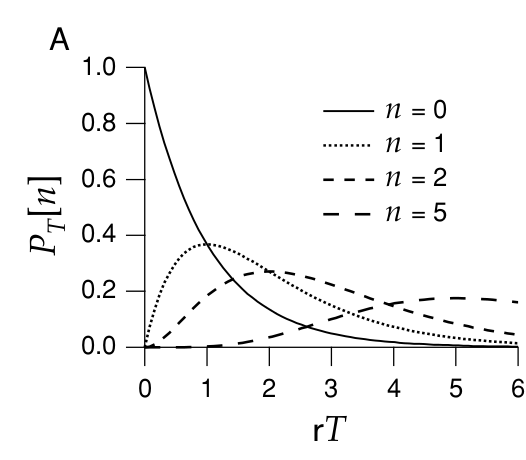
\includegraphics[scale = 0.2]{png/Figure1-11-A}\\        
        \label{fig:1.11}            
\end{center}

\begin{exm}
    Figure \ref{fig:1.12} shows the probabilities of various numbers of spikes occurring when the average number of spikes is 10.For large rT,which corresponds to a large expected number of spikes, the Poisson distribution approaches a Gaussian distribution with mean and variance equal to rT.Figure \ref{fig:1.12} shows that this approximation is already quite good for rT = 10.
\end{exm}    

\begin{center}
    % 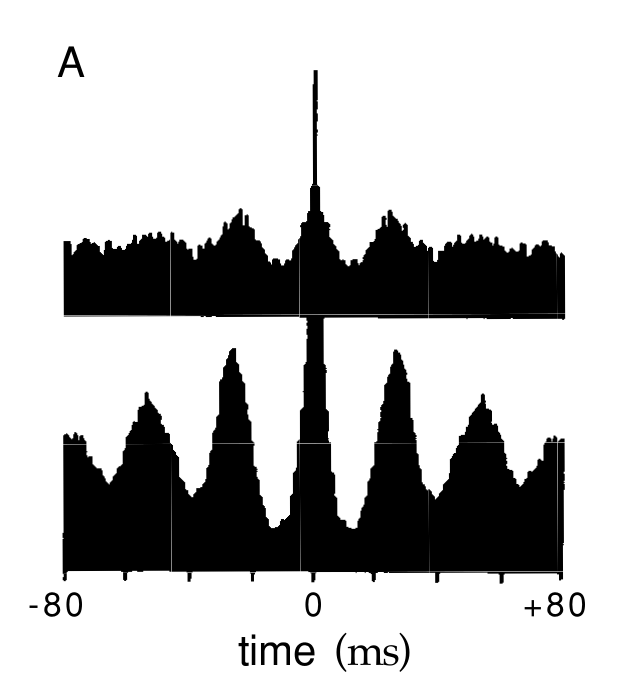
\includegraphics[scale = 0.2]{png/Figure1-12-A}\\
    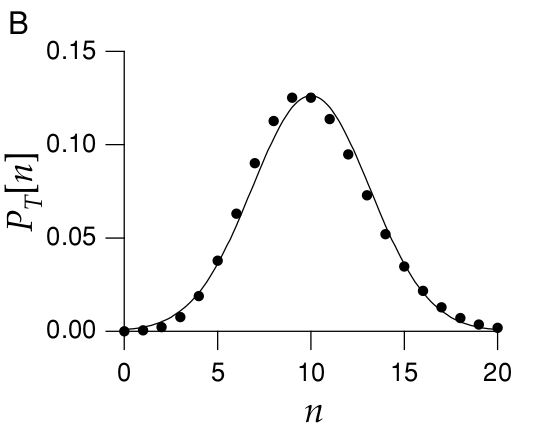
\includegraphics[scale = 0.2]{png/Figure1-11-B}\\    
    \label{fig:1.12}        
\end{center}

\begin{thm}
    The probability $P[t_1,t_2,...,t_n]$can be expressed in terms of another probability function $P_T[n]$,which is the probality that an arbitrary sequence of exactly n spikes occurs within a trial of duration T.Assuming that the spike times are ordered so that $0\leq t_1\leq t_2\leq ...\leq t_n\leq T$,the relationship is 
    \begin{equation}
        P[t_1,t_2,...,t_n]=n!{_T[n](\frac{\vartriangle t}{T})^n}
        \label{eq:1.26}
    \end{equation}
    \begin{proof}
    \end{proof}
\end{thm}

\begin{coro}
    We can compute the variance of spike counts produced by a Poisson process from the probabilities in equation \ref{eq:1.29}.The spike count is $$\sigma^2_n = \langle n^2 \rangle -\langle n  \rangle ^2=rT $$
\end{coro}

\begin{defn}
    % (Fano factor)The ratio of the variance and mean of the spike count ,$\sigma^2_n/\langle n\rangle$,is called the Fano factor.
    The ratio of the variance and mean of the spike count ,$\sigma^2_n/\langle n\rangle$,is called the Fano factor.    
\end{defn}

\begin{coro}
    The Fano factor takes the value 1 for a homogeneous Poisson process,independent of the time interval T.
\end{coro}

\begin{lem}
    % For a homogeneous Poisson process,the probability of an interspike intervalfalling between $\tau$ and $\tau + \vartriangle t$ is $$P[\tau\leq t_{i+1}-t_{i}<\tau +\vartriangle t]=r\vartriangle t\ exp(-r\tau)$$.
    the probability of an interspike intervalfalling between $\tau$ and $\tau + \vartriangle t$ is 
    \begin{equation}
        P[\tau\leq t_{i+1}-t_{i}<\tau +\vartriangle t]=r\vartriangle t\ exp(-r\tau)
        \label{eq:1.31}
    \end{equation}
    \begin{proof}
    \end{proof}
\end{lem}

\begin{thm}
    From the interspike interval distribution of a homogeneous Poisson spike train , we can compute the mean interspike interval,
    \begin{equation}
        \langle \tau \rangle =\int^{\infty}_{0}\tau r\ exp(-r\tau)d\tau  = \frac{1}{r}
        \label{eq:1.32}         
    \end{equation}
    and the variance of the interspike intervals,
    \begin{equation}
        \sigma^2_\tau =\int^{\infty}_{0}\tau^2 r\ exp(-r\tau)d\tau - \langle \tau \rangle^2 = \frac{1}{r^2}
        \label{eq:1.33}         
    \end{equation}
\end{thm}

\begin{defn}
    The ratio of the standard deviation to the mean
    \begin{equation}
        C_V=\frac{\sigma}{\langle \tau  \rangle}
        \label{eq:1.34}
    \end{equation} is called the coefficient of variation.
\end{defn}

\begin{rem}
    The coefficient of variation takes the value 1 for a homogeneous Poisson process.This is a necessary, though not sufficient,condition to identify a Poisson spike train.Recall that the Fano factor for a Poisson process is also 1.For any renewal process,the Fano factor evaluated over long time intervals approaches the value $C^2_V$
\end{rem}

\subsection{The Spike-Train Autocorrelation Funciton}

\begin{lem}
    The spike-train autocorrelation function is 
    \begin{equation}
        Q_{\rho\rho}(\tau)=\frac{1}{T}\int^T_0 \langle (\rho(t)-\langle r \rangle)(\rho(t+\tau)-\langle r\rangle)\rangle
        \label{eq:1.35}
    \end{equation}
    \begin{proof}
    \end{proof}
\end{lem}
    
\begin{center}
    \label{fig:1.12A}    
    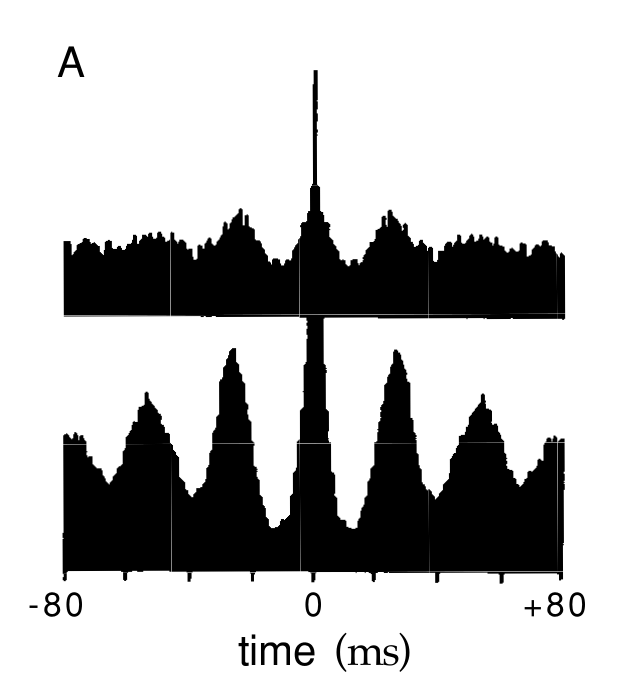
\includegraphics[scale = 0.2]{png/Figure1-12-A.png}\\
\end{center}

\begin{center}
    \label{fig:1.12B}    
    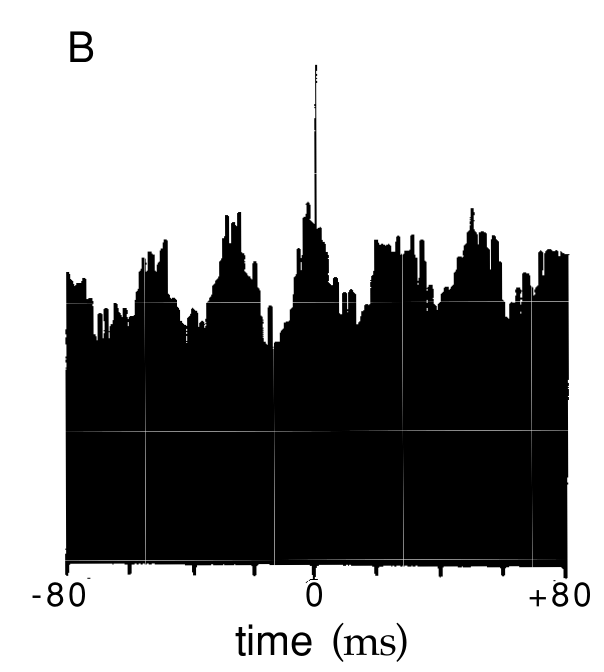
\includegraphics[scale = 0.2]{png/Figure1-12-B.png}\\
\end{center}

\begin{center}
    \label{fig:1.13A}    
    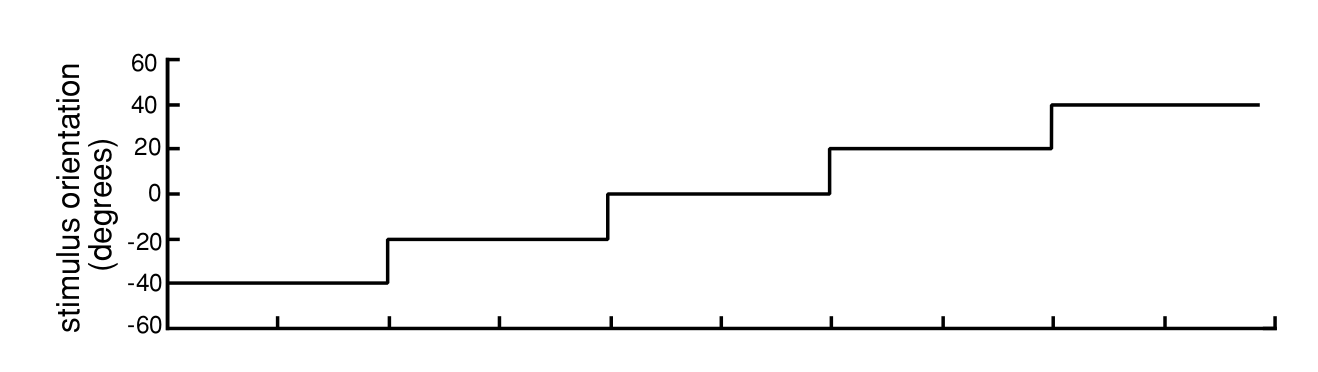
\includegraphics[scale = 0.2]{png/Figure1-13-A.png}\\
\end{center}

\begin{center}
    \label{fig:1.13B}    
    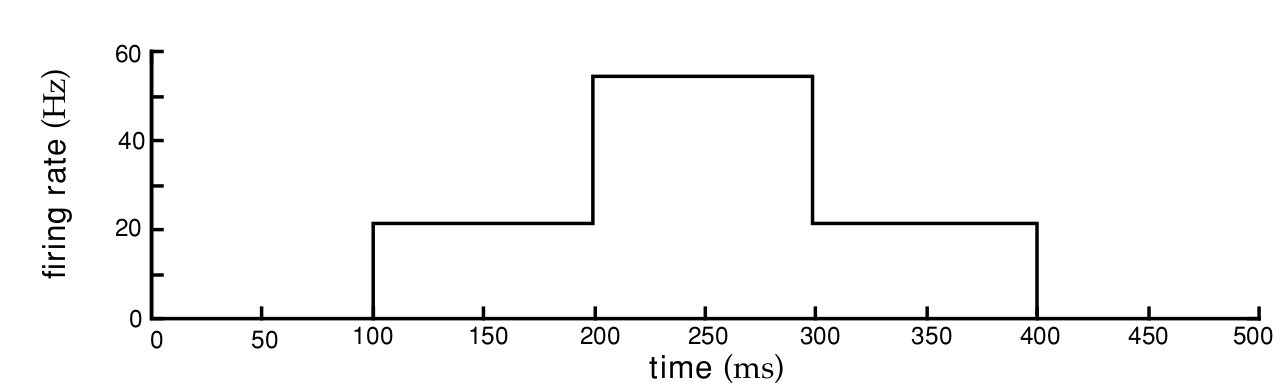
\includegraphics[scale = 0.2]{png/Figure1-13-B.png}\\
\end{center}

\begin{center}
    \label{fig:1.13C}    
    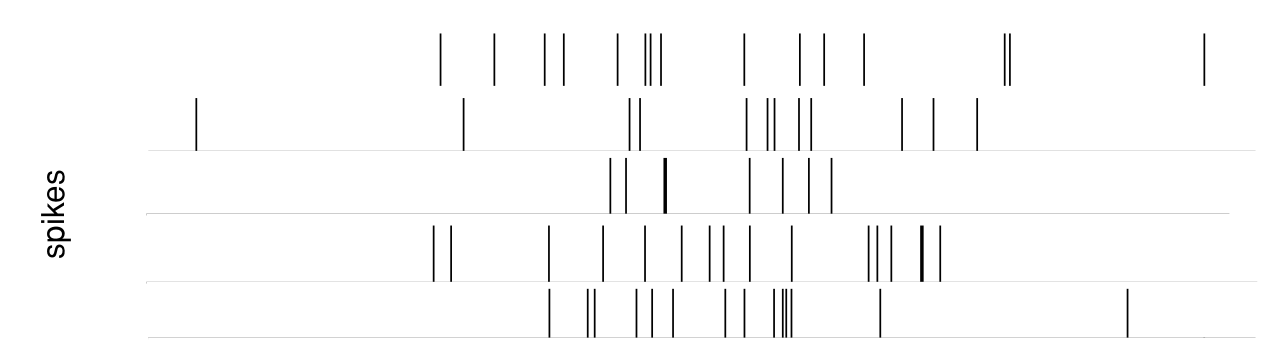
\includegraphics[scale = 0.2]{png/Figure1-13-C.png}\\
\end{center}

\begin{center}
    \label{fig:1.14A}    
    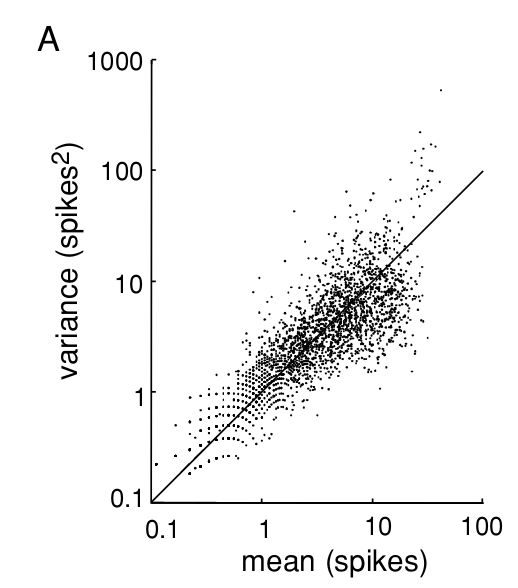
\includegraphics[scale = 0.2]{png/Figure1-14-A.png}\\
\end{center}

\begin{center}
    \label{fig:1.14B}    
    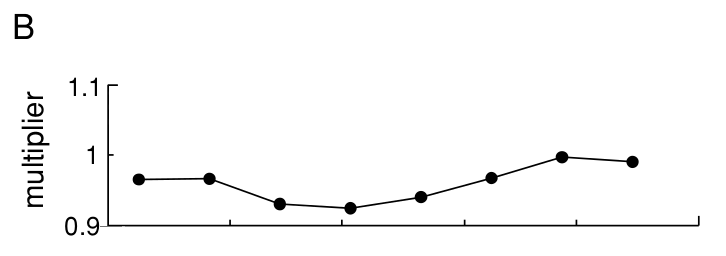
\includegraphics[scale = 0.2]{png/Figure1-14-B.png}\\
\end{center}

\begin{center}
    \label{fig:1.14C}    
    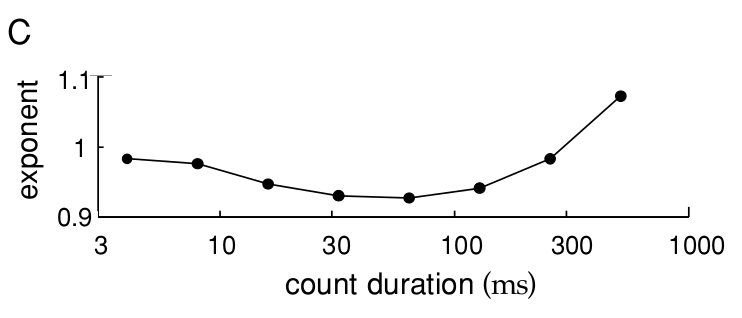
\includegraphics[scale = 0.2]{png/Figure1-14-C.png}\\
\end{center}

\begin{center}
    \label{fig:1.15A}    
    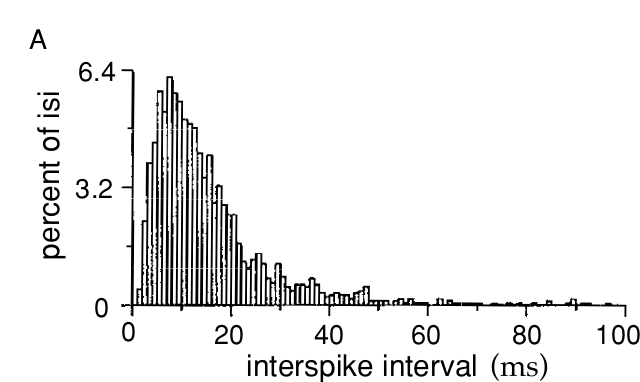
\includegraphics[scale = 0.2]{png/Figure1-15-A.png}\\
\end{center}

\begin{center}
    \label{fig:1.15B}    
    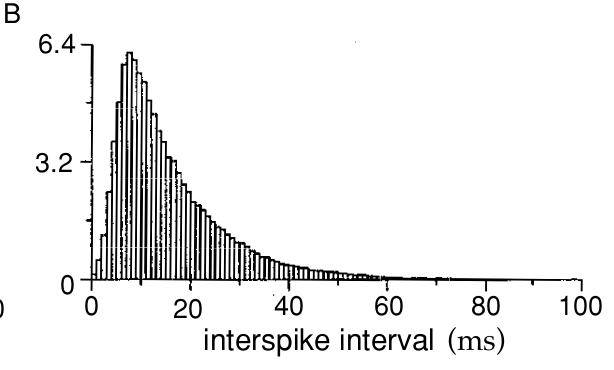
\includegraphics[scale = 0.2]{png/Figure1-15-B.png}\\
\end{center}

\begin{center}
    \label{fig:1.16}    
    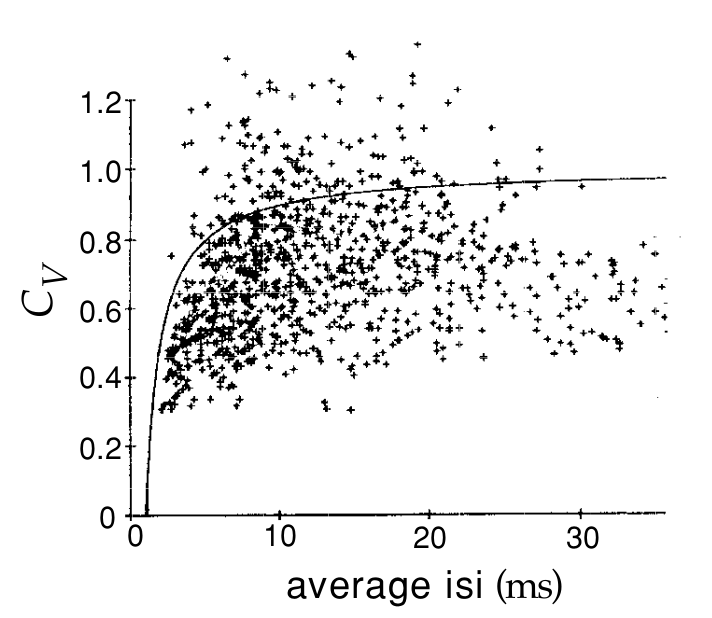
\includegraphics[scale = 0.2]{png/Figure1-16.png}\\
\end{center}







% problem: 图像无法正确索引
